
\documentclass[a4paper,11pt]{article}%,twocolumn
%% packages

\usepackage{blindtext} % needed for creating dummy text passages
%\usepackage{ngerman} % needed for German default language
\usepackage{amsmath} % needed for command eqref
\usepackage{amssymb} % needed for math fonts
\usepackage[colorlinks=true,breaklinks]{hyperref} % needed for creating hyperlinks in the document, the option colorlinks=true gets rid of the awful boxes, breaklinks breaks lonkg links (list of figures), and ngerman sets everything for german as default hyperlinks language
\usepackage[hyphenbreaks]{breakurl} % ben�tigt f�r das Brechen von URLs in Literaturreferenzen, hyphenbreaks auch bei links, die �ber eine Seite gehen (mit hyphenation).
\usepackage{xcolor}
\definecolor{c1}{rgb}{0,0,1} % blue
\definecolor{c2}{rgb}{0,0.3,0.9} % light blue
\definecolor{c3}{rgb}{0.3,0,0.9} % red blue
\hypersetup{
    linkcolor={c1}, % internal links
    citecolor={c2}, % citations
    urlcolor={c3} % external links/urls
}
%\usepackage{cite} % needed for cite
\usepackage[square,authoryear]{natbib} % needed for cite and abbrvnat bibliography style
\usepackage[nottoc]{tocbibind} % needed for displaying bibliography and other in the table of contents
\usepackage{graphicx} % needed for \includegraphics 
\usepackage{longtable} % needed for long tables over pages
\usepackage{bigstrut} % needed for the command \bigstrut
\usepackage{enumerate} % needed for some options in enumerate
%\usepackage{todonotes} % needed for todos
\usepackage{makeidx} % needed for creating an index
\makeindex
\usepackage{gensymb}
\usepackage{url}
\usepackage{psfrag}
\usepackage{multirow}
\usepackage{subfigure}
%% page settings

\usepackage[top=20mm, bottom=20mm,left=15mm,right=15mm]{geometry} % needed for page border settings
\parindent=0mm % for space of first line of new text block
\sloppy % for writing with hyphenless justification (tries to)
\hyphenation{} % use hyphenation of tolerance parametershttp://www.jr-x.de/publikationen/latex/tipps/zeilenumbruch.html
\hyphenpenalty=10000
\exhyphenpenalty=10000
\usepackage{fancyhdr} % needed for head and foot options
%% my macros

%% Text fomats
\newcommand{\tbi}[1]{\textbf{\textit{#1}}}

%% Math fonts
\newcommand{\bbA}{\mathbb{A}}
\newcommand{\bbB}{\mathbb{B}}
\newcommand{\bbC}{\mathbb{C}}
\newcommand{\bbD}{\mathbb{D}}
\newcommand{\bbE}{\mathbb{E}}
\newcommand{\bbF}{\mathbb{F}}
\newcommand{\bbG}{\mathbb{G}}
\newcommand{\bbH}{\mathbb{H}}
\newcommand{\bbI}{\mathbb{I}}
\newcommand{\bbJ}{\mathbb{J}}
\newcommand{\bbK}{\mathbb{K}}
\newcommand{\bbL}{\mathbb{L}}
\newcommand{\bbM}{\mathbb{M}}
\newcommand{\bbN}{\mathbb{N}}
\newcommand{\bbO}{\mathbb{O}}
\newcommand{\bbP}{\mathbb{P}}
\newcommand{\bbQ}{\mathbb{Q}}
\newcommand{\bbR}{\mathbb{R}}
\newcommand{\bbS}{\mathbb{S}}
\newcommand{\bbT}{\mathbb{T}}
\newcommand{\bbU}{\mathbb{U}}
\newcommand{\bbV}{\mathbb{V}}
\newcommand{\bbW}{\mathbb{W}}
\newcommand{\bbX}{\mathbb{X}}
\newcommand{\bbY}{\mathbb{Y}}
\newcommand{\bbZ}{\mathbb{Z}}
\usepackage[ framed, numbered]{matlab-prettifier}%framed,%
\usepackage{listings}
\usepackage{physics}
\usepackage{pdfpages}
\usepackage[toc,page]{appendix}
\usepackage{float}

\begin{document}
\begin{titlepage}
\center % Center everything on the page

%-------------------------------------------------------------------------------------
%	HEADING SECTIONS
%------------------------------------------------------------------------------------
\textbf{\large Department of Electrical and Computer Engineering}\\[0.5cm]
\textbf{\Large University of Colorado at Boulder}\\[1cm]
\textbf{\large ECEN5730 - Practical PCB design}\\[2cm]

\includegraphics[width=0.3\textwidth]{figures/cu}\\[2cm] 

	
%-------------------------------------------------------------------------------------
%	TITLE SECTION
%------------------------------------------------------------------------------------

\textbf{\Huge Board Good Layout/Bad Layout }\\[0.2cm]

\textbf{\Large Report}\\[2cm]
\vspace{1.5cm}
\begin{figure}[H]
	\centering
	
\includegraphics[scale=0.2]{figures/qr_download.png}
	\label{555_schematic}
\end{figure}\vspace{1.5cm}


%----------------------------------------------------------------------------------------
%	MEMBERS SECTION
%----------------------------------------------------------------------------------------


\vfill

\textbf{\large Submitted by}

{\large Parth Thakkar}\\[0.5cm]




%----------------------------------------------------------------------------------------
%	DATE SECTION
%----------------------------------------------------------------------------------------

\textbf{\large Submitted on}\\
\textbf{\Large \today} % Date, change the \today to a set date if you want to be precise

%----------------------------------------------------------------------------------------

\vfill % Fill the rest of the page with whitespace

\end{titlepage}

\pagebreak

\tableofcontents
\listoffigures
\listoftables
\vfill
\begin{center}
	\textbf{\textit{*PDF is clickable}}
\end{center}

\pagebreak

\section{Objective / Purpose of Lab}

The goal of this laboratory exercise is to build and analyze a circuit using two types of 555 timer ICs, one fast and one slow. The main tasks include:

\begin{enumerate}
	\item Construct a circuit with a fast 555 timer IC, and then replace it with a slow 555 timer IC. Observe and compare the rise and fall times of the output signals, the waveform shapes, and the output voltage levels in two scenarios: driving an open circuit and driving a circuit with a 50 ohm resistor and LED in series.
	\item Modify the circuit to drive an LED using three different series resistors: 50 ohms, 1k ohms, and 10k ohms. Record the differences in the output voltage for each resistor value.
	\item Using an oscilloscope with a 10x probe, measure the rise and fall time of the 555 timer output for each IC type, both with and without the 50 ohm resistor and LED. Also, determine the frequency and duty cycle of the output signal. These measurements should first be estimated visually before using the scope’s cursor or measurement functions for accuracy.
	\item Compare the observed values with the predicted values for frequency and duty cycle, noting any significant differences or insights gained.
\end{enumerate}


This exercise aims to develop a practical understanding of the 555 timer IC's behavior in different configurations and load conditions.

here is block diagram of the system,

\begin{figure}[!h]
	\centering
	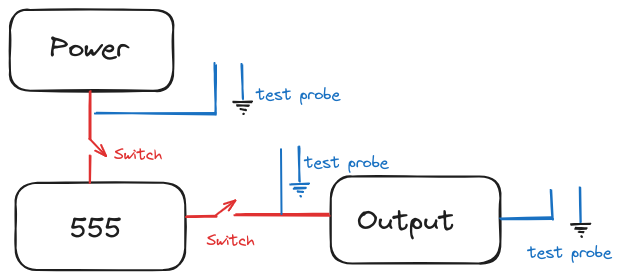
\includegraphics[scale=0.4]{figures/ne555_blockdiagram}
	\caption{Idealized frequency response of a Bandpass}
	\label{idealbpfilter}
\end{figure}
\pagebreak

\section{Component listing}


\begin{table}[!h]
	\centering

	\begin{tabular}{l c c c}
		\hline
		\textbf{Component Name}&\textbf{Usecase}&\textbf{Symbol}&\textbf{Value}\\\hline
		&&\\
1 x Capacitor&Charging Discharging Capacitor&C5&0.1$\mu$F\\
1 x Capacitor&Decoupling cap&C5&22$\mu$F\\
1 x Capacitor&Filter Capacitor&C5&10$\mu$F\\
1 x Potentiometer&Change the Waveform Dutycycle&R2&10k$\ohm$\\
1 x Resistor&Discharging rate Resistor&R3&15k$\ohm$\\
1 x Resistor&Current Limiting resistor&R4&50$\ohm$\\
1 x Resistor&Current Limiting resistor&R5&300$\ohm$\\
1 x Resistor&Current Limiting resistor&R6&1k$\ohm$\\
1 x Resistor&Current Limiting resistor&R7&10k$\ohm$\\
1x NE555&Timer IC&U1\\
1 x Diode&Discharging bypass Diode&D1\\
3 x Switch&To isolate the Circuit&SW\\
3 x LEDs&For output&LED\\
\hline\hline
	\end{tabular}
	\caption{Prescribed Filter specifications}
	\label{filterspecs}
\end{table}



\section{Napkin Sketch}

Circuit given in the lab manual can give us approx 60\% 
of duty cycle, So I have come up with my circuit to make the circuit work at 50\% duty cycle and also be able to vary the circuit

for simple circuit we can see that the overall time for one cycle would be
\begin{flalign*}
	& T_{total} = T_{charging} + T_{discharging}&& \\\\
	& \textbf{And expanding each timing term would give us,}&& \\
	&T_{charging} = 0.693 \cdot(R_1 + R_2) \cdot C&& \\
	& T_{discharging} = 0.693 \cdot(R_2) \cdot C&& \\\\
	&\textbf{so the total time for charging and Discharging would be, }&& \\
	&T_{total} = 0.693 \cdot(R_1 + R_2) \cdot C + 0.693 \cdot(R_2) \cdot C&& \\
	&T_{total} = 0.693 \cdot(R_1 +  2 \cdot R_2) \cdot C&& \\
\end{flalign*}



I have used bypass diode to remove resistance R2 while discharging the Capacitor so R2 would be removed from the equation and equation would become just,
\begin{flalign*}
&T_{charging} = 0.693 \cdot(R_1 + R_2) \cdot C&& \\
&T_{discharging} = 0.693 \cdot C&& \\\\
&T_{total} = 0.693 \cdot(R_1 + R_2) \cdot C&& \\
\end{flalign*}

Here is the schematic with bypass diode to reduce the time 
for discharging the cap
\begin{figure}[!h]
	\centering
	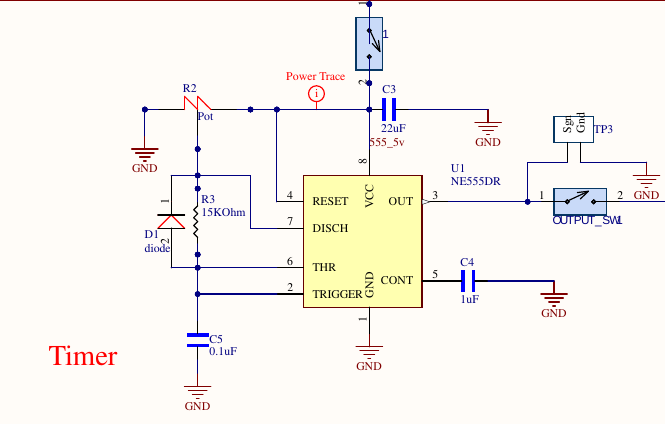
\includegraphics[scale=0.8]{figures/timer_sch}
	\caption{Schematic for variable duty-cycle 555 Timer}
	\label{555_schematic}
\end{figure}

\pagebreak
\section{Calculations}

Equation for schematic with bypass diode is,
\begin{gather}
	T_{total} = 0.693 \cdot(R_1 + R_2) \cdot C
\end{gather}

We need 50\% duty cycle so we will assume that $T_{charging}$ and $T_{discharging}$ is same.
\begin{flalign*}
	& T_{charging} = T_{discharging}&& \\
	& 0.693 \cdot(R_1 + R_2) \cdot C = 0.693 \cdot C&& \\
	& R_1 = R_2 \textit{(negative sign implies Current in reverse direction)}
\end{flalign*}

We need 500Hz frequency and we are assuming C as 0.1$\mu$F putting this value in the equation and putting $R_1 = R_2$ 	
\begin{flalign*}
	& T_{total} = 0.693 \cdot(R_1 + R_2) \cdot C && \\
	& \left(\frac{1}{500} \right) = 0.693 \cdot(R_1 + R_2) \cdot C && \\
	& \left( \frac{0.002}{0.693} \right) = 2 \cdot R_1 \cdot 0.1 \cdot 10^{-6} && \\
	& \boxed{R_1 = 15k\ohm} && \\
\end{flalign*}

So, I have added $R_2$ as 15k ohm and $R_1$ is variable Potentiometer of 10k$\ohm$ so that we can change the output frequency.

\pagebreak
\section{Scope shots with analysis}

Below Schematic \ref{cap} shows charging discharging of capactor at constant rate, it shows that it will start charging at 1/3 V and start discharging at 2/3 V .
\begin{figure}[!h]
	\centering
	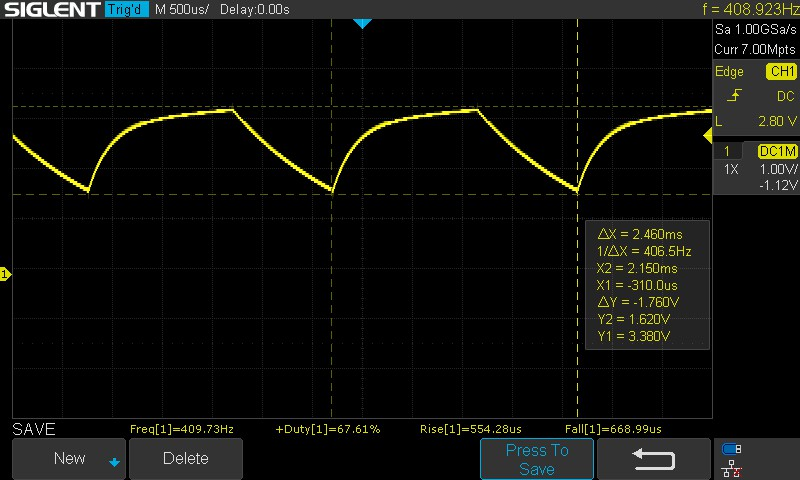
\includegraphics[scale=0.6]{figures/cap}
	\caption{Capacitor Charging and Discharging}
	\label{cap}
\end{figure}

Below referance scope image \ref{overall_duty_cycle} is denoting frequency of 499.22Hz and duty cycle of 48\% with setting potentiometer to match $R_2$ that is 15k.
\begin{figure}[!h]
	\centering
	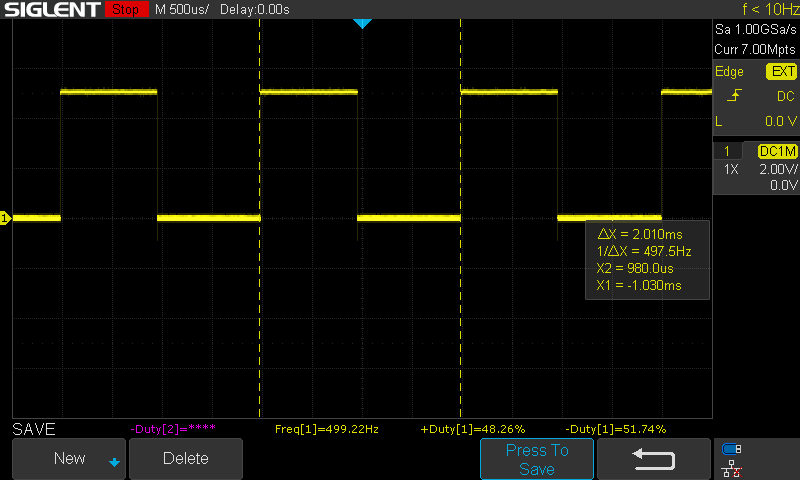
\includegraphics[scale=0.5]{figures/overall_duty_cycle.png}
	\caption{Duty cycle after setting potentiometer to set at 15k}
	\label{overall_duty_cycle}
\end{figure}


Here you can see in the image \ref{555_slow} the rise and fall time of \textbf{Fast} 555 timer IC is around 30ns and 40ns.
\begin{figure}[H]
	\centering
	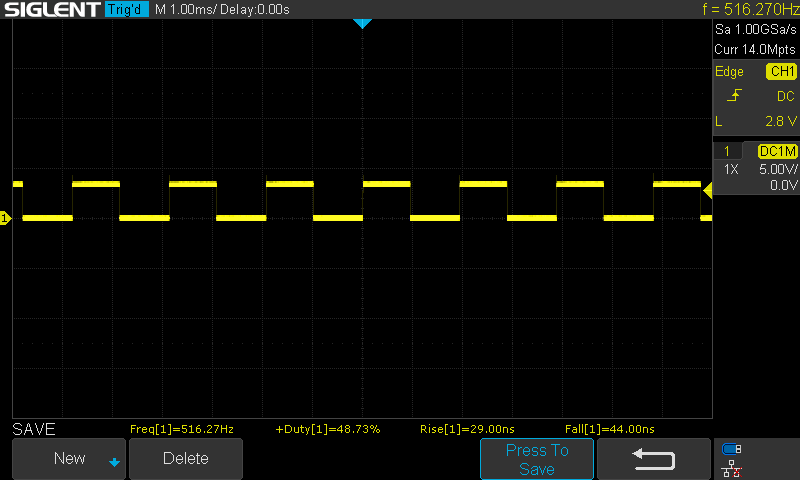
\includegraphics[scale=0.5]{figures/555_slow}
	\caption{scope capture for rise and fall time for Fast NE555}
	\label{555_slow}
\end{figure}


Here you can see in the image \ref{555_slow} the rise and fall time of \textbf{Slow} 555 timer IC is around 30ns and 22ns.


\begin{figure}[H]
	\centering
	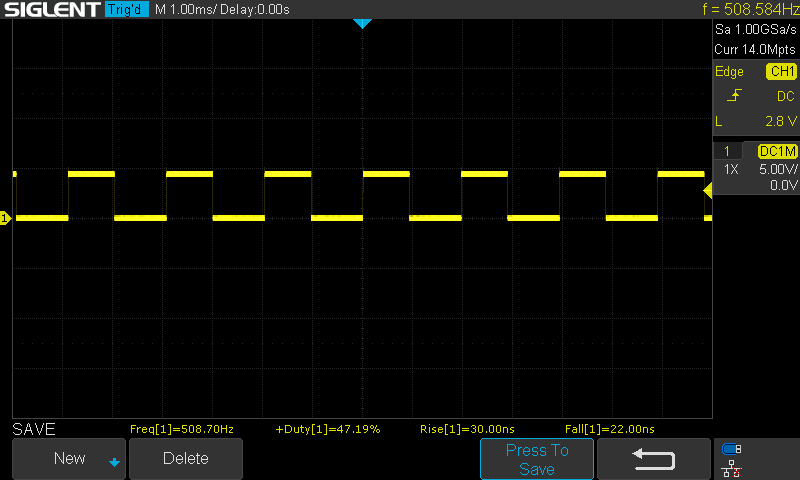
\includegraphics[scale=0.5]{figures/555_fast}
	\caption{scope capture for rise and fall time for Slow NE555}
	\label{555_fast}
\end{figure}


After setting knob to highest resistance we can see that the duty cycle increases to max of around 92\%. see image \ref{90_duty}
\begin{figure}[H]
	\centering
	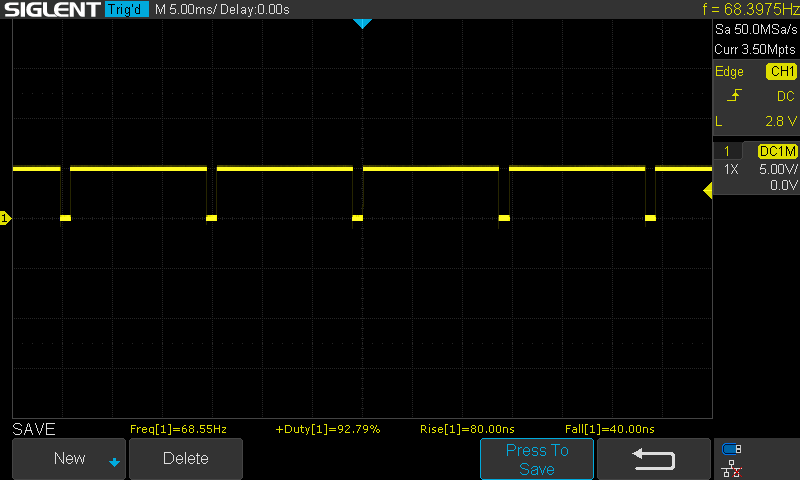
\includegraphics[scale=0.6]{figures/90_duty}
	\caption{duty cycle = 92\%}
	\label{90_duty}
\end{figure}

After setting knob to highest resistance we can see that the duty cycle increases to max of around 92\%. see image \ref{0_duty}
\begin{figure}[H]
	\centering
	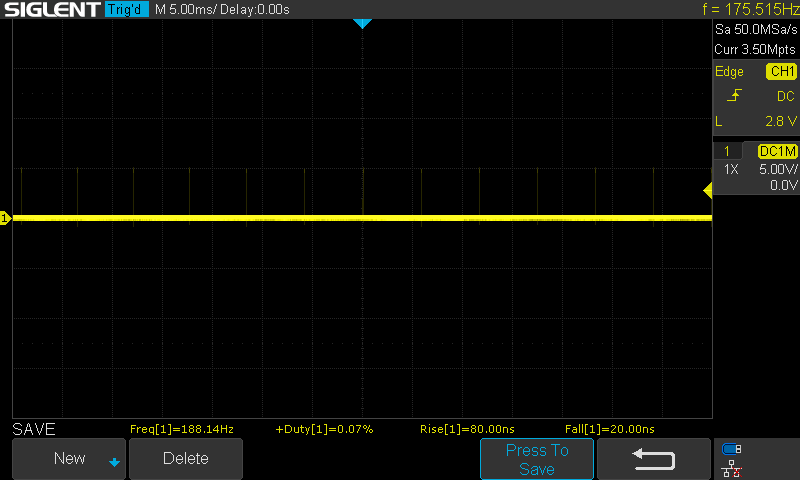
\includegraphics[scale=0.6]{figures/0_duty}
	\caption{duty cycle = 0.07\%}
	\label{0_duty}
\end{figure}


Also for the Current Consumption here is the

\begin{table}[H]
	\centering

	\begin{tabular}{l c c}

		\textbf{Component Name}&\textbf{Rise Time}&\textbf{Fall Time}\\\hline
		&&\\
		\textbf{NE555 fast}&29ns&22ns\\
		\textbf{NE555 slow}&30ns&44ns\\

	\end{tabular}
	\caption{Rise-time and Fall-time}
	\label{tab_rise_fall}
\end{table}

and Rise time and fall time for both IC is mentioned below

\begin{table}[H]
	\centering

	\begin{tabular}{l c c c}
		\textbf{}&\textbf{50$\ohm$}&\textbf{1k$\ohm$}&\textbf{10k$\ohm$}\\\hline
		&&\\
		\textbf{Current}&3.11 mA&728 $\mu$A&94 $\mu$A\\
		\textbf{Voltage}&2.630 V&2.745 V&2.847V\\
	\end{tabular}
	\caption{Current Consumption}
	\label{tab_curent_consumption}
\end{table}

This is happening as the datasheet suggest that the slow 555 would give large current draw and current sink in the output and fast one will have faster rise time and fall time but it would not be able to draw much current, more that 50mA from output
\pagebreak

\section{Conclusion}

The lab demonstrated the characteristics of 555 timer ICs in various configurations. The primary objectives were met. And creating 2 layer PCB with understanding of how to use altium, debug the PCB and use theoretical knowledge to create it in software.

\begin{enumerate}
	\item \textbf{Circuit Construction and Analysis:}\\
	Observations showed distinct differences in the rise and fall times, waveform shapes, and output voltage levels when driving both an open circuit and a circuit loaded with a 50 ohm resistor and LED in series.
	\item \textbf{LED Driving with Variable Resistors:}\\
	Driving an LED with 50 ohm, 1k ohm, and 10k ohm resistors highlighted the impact of varying resistance on the output voltage. This variation was to understand the relationship between resistance and voltage.
	\item \textbf{Extra:} \\
	Manipulating the duty cycle using a potentiometer and a bypass diode, achieving a 50\% duty cycle, as well as extremes near 0\% and 92\%, demonstrated the range of operation and the effects of resistance changes on the duty cycle. 
	\item \textbf{Current Consumption Analysis:}\\
	The slow 555 IC showed a higher current draw capability, aligning with datasheet specifications, whereas the fast 555 IC exhibited quicker rise and fall times but limited current draw capability.
	\item \textbf{Integrating PCB Design into Learning:}\\
	The development of a 2-layer PCB Adding Test probe for voltage measurement and how to isolate the different part of circuit for debugging purpose in the pcb design.
   
\end{enumerate}

Breadboard Implementation:

\begin{figure}[H]
	\centering
	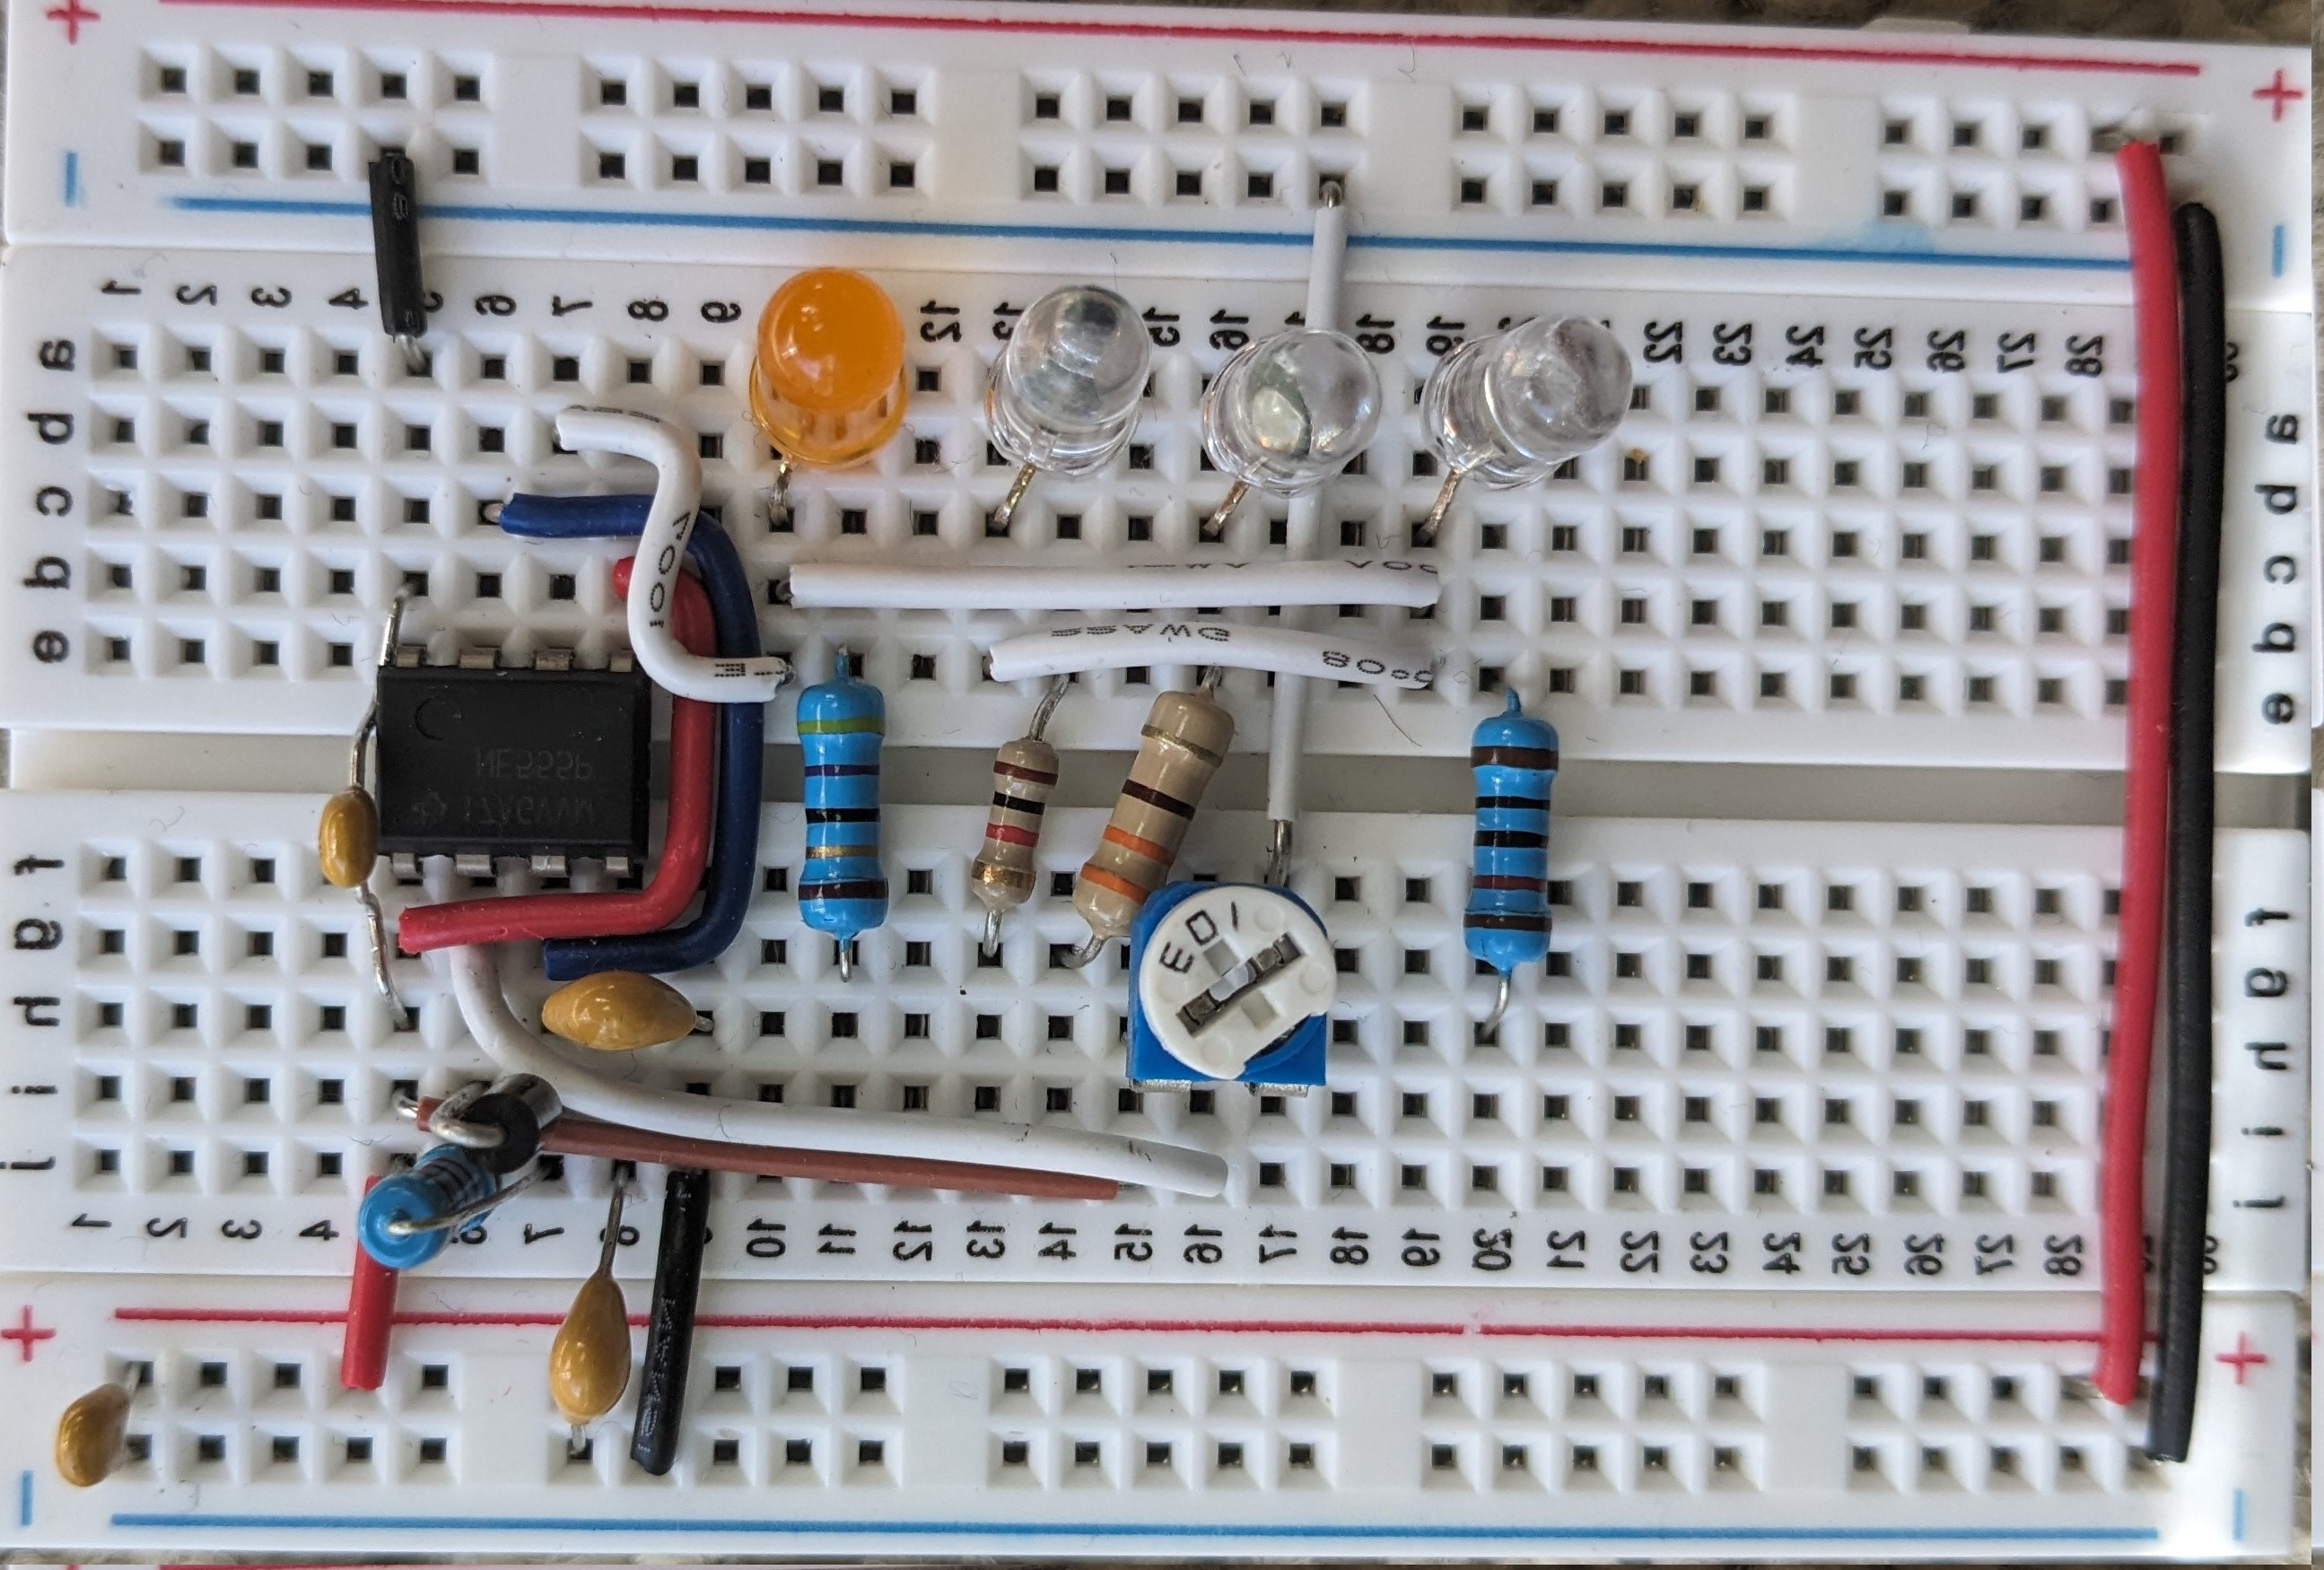
\includegraphics[scale=0.2]{figures/breadboard.jpg}
	\caption{Breadboard Implementation}
	\label{breadboard}
\end{figure}

Here is the PCB design for top layer and bottom layer:

\begin{figure}[H]
	\centering
	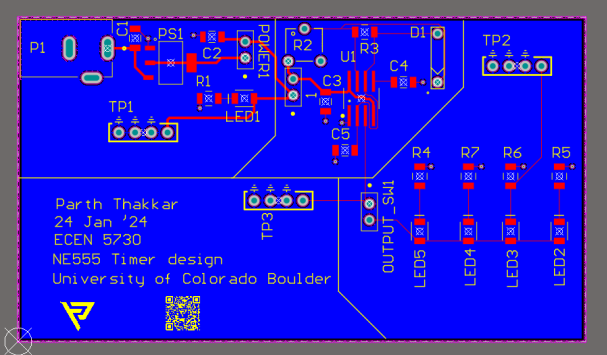
\includegraphics[scale=0.8]{figures/top.png}
	\caption{Top layer PCB}
	\label{top}
\end{figure}

\begin{figure}[H]
	\centering
	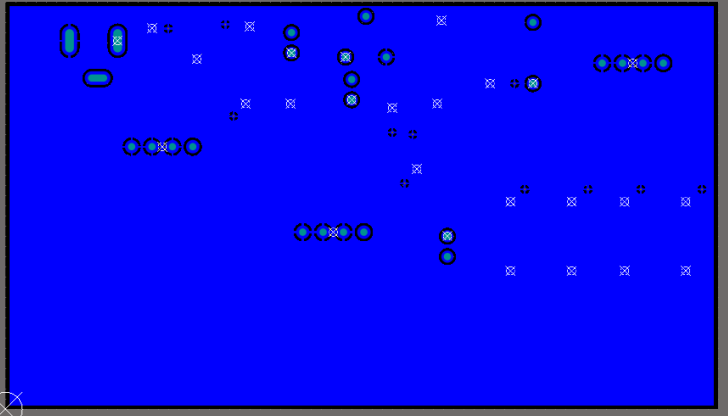
\includegraphics[scale=0.8]{figures/bottom.png}
	\caption{Bottom Layer PCB}
	\label{bottom}
\end{figure}



\vfill
\hrule
\vspace{0.5cm}



\vspace{1cm}
\hrule
\vspace{0.5cm}


%---------------------------------------------------------------------------
\end{document}
-
